\documentclass[11pt]{article}
\usepackage[margin=1in]{geometry}
\usepackage{graphicx}
\usepackage{booktabs}
\usepackage{amsmath}
\usepackage{hyperref}
\usepackage{natbib}
\usepackage{xcolor}
\usepackage{caption}
\captionsetup{font=small,labelfont=bf}

\title{What does language grounding actually contribute to cell
  representations?\\ A controlled decomposition on held-out donors}
\author{A.~I.~Robles\thanks{Corresponding author. Code and artifacts:
  \url{https://github.com/alrobles/biocellAI}}\\
  Department of Ecology \& Evolutionary Biology, University of Kansas}
\date{Draft — \today}

\begin{document}
\maketitle

\noindent\textbf{Scientific audit status: not submission-ready.}
This draft retains historical exploratory results from protocol v1. ADR-011
specifies a corrective revalidation programme; no corrected v2 results are
reported here yet. Historical claims of label-free training, strict zero-shot
transfer, semantic attribution and causal composition/state decomposition are
not established. The results sections below must be re-evaluated before those
claims or gate decisions can be used in a submission.

\begin{abstract}
What does biological language contribute beyond the supervision used to
assign text to cells? We assembled an exploratory benchmark spanning Tabula
Sapiens blood, SEA-AD neuropathology and an external ROSMAP cohort. Historical
blood experiments recorded macro-F1 of 0.591 for marker-caption alignment
versus 0.603 for a supervised reference; external-marker retrieval and synthesis
recorded similar performance. These are \emph{text-mediated supervised}
experiments: class annotations assign captions even when their wording omits
the class name. Caption register strongly affected nearest-prototype scoring.
Historical SEA-AD analyses recorded donor CPS correlations near 0.60, while
tested scGPT fine-tuning configurations did not improve that result. A
composition-only diagnostic recorded approximately 0.50. These observations
do not yet identify a language-specific or within-cell-type state advantage.
A methodological audit identified repeated preprocessing, reuse of fold-derived
captions, transductive PCA, target-label orientation in transfer and
non-equivalent foundation-model input protocols. We therefore distinguish
historical observations from a corrective revalidation programme using frozen
donor splits, train-only transformations, label-equivalent non-text controls,
paired donor-level inference and biological review of captions. Conclusions
about semantic benefit, strict transfer and encoder scale remain conditional
on that revalidation; this draft reports no corrected v2 results.
\end{abstract}

\section{Introduction}

Single-cell foundation models --- scGPT \citep{scgpt}, Geneformer
\citep{geneformer}, scFoundation \citep{scfoundation} and successors ---
learn cell representations from expression profiles alone. A parallel line
of work argues that grounding those representations in biological language
unlocks generalization that molecular data alone cannot provide:
CellWhisperer aligns transcriptomes with AI-curated textual annotations
\citep{cellwhisperer}, C2S-Scale renders expression profiles as ``cell
sentences'' inside a general-purpose LLM \citep{c2sscale}, and ongoing open
efforts (e.g., the Allen Institute's CellOLMo direction on top of OLMo
\citep{olmo}) aim to build multimodal models where text is a first-class
modality rather than an annotation.

The motivating question --- \emph{does language grounding improve cell
representations?} --- is harder to answer than it looks, because
``grounding'' bundles at least three distinct mechanisms: (i) text can carry
\emph{label-discriminative structure} (captions derived from cell-type
labels); (ii) text can carry \emph{external biological knowledge}
(function, lineage, marker semantics); and (iii) text can act as a
\emph{representation bottleneck} that smooths per-cell measurement noise.
Published systems typically report end-to-end performance and leave the
decomposition implicit.

Here we isolate these mechanisms with a deliberately small, controlled
experiment. On 85{,}055 human blood cells from Tabula Sapiens
\citep{tabulasapiens} accessed via CZ CELLxGENE Census
\citep{cellxgene}, we train the same cell encoder either end-to-end with
labels (supervised baseline) or by contrastive alignment to four different
caption sources, and evaluate all models on \emph{whole held-out donors}
with no label access at inference. Our contributions:

\begin{enumerate}
  \item A reproducible benchmark protocol for language-grounded cell
    representations with donor-level held-out evaluation and explicit
    leakage probes.
  \item Evidence that zero-shot cell-type assignment via marker-list
    grounding reaches supervised performance on unseen donors
    (0.591 vs.\ 0.603 macro-F1), showing that contrastive text alignment
    can carry class structure across individuals.
  \item A decomposition showing this benefit is carried almost entirely by
    label-derived discriminative text: label-free grounding sources
    (per-cell gene lists, LLM-inferred prose) recover only 48--66\% of the
    marker-list result, and a biomedical text encoder offers no advantage
    on gene-list captions.
  \item A cautionary engineering finding: identifier-mapping errors
    (Ensembl/positional feature IDs in place of gene symbols) silently
    destroy grounding semantics --- a failure mode that produced
    measurable metric differences and is now pinned by regression tests.
\end{enumerate}

\section{Related work}

\paragraph{Expression-only single-cell foundation models.}
scGPT \citep{scgpt}, Geneformer \citep{geneformer}, scFoundation
\citep{scfoundation}, and UCE \citep{uce} learn cell representations from
expression alone; UCE additionally targets cross-species universality via
protein-embedding gene tokens. Critically, independent zero-shot
evaluations find these models underperform simple baselines
\citep{kedzierska,scfm_limits}: \citet{kedzierska} show Geneformer and
scGPT lose to HVG selection plus Harmony/scVI on cell-type clustering, and
\citet{scfm_limits} report Seurat v5 beating all three on classification.
The burden of proof for any added modality is therefore high --- motivating
the controlled, leakage-aware protocol used here.

\paragraph{Language-grounded cell models.}
LangCell \citep{langcell} established contrastive cell--text pretraining
on metadata-derived captions; CellWhisperer \citep{cellwhisperer} scales
CLIP-style alignment to $\sim$1M cells with AI-curated descriptions and
adds a chat interface; C2S-Scale \citep{c2sscale} and Cell2Sentence
\citep{cell2sentence} instead serialize expression as ``cell sentences''
inside general LLMs. None of these decompose which part of the text
carries the transferable signal --- our central question.

\paragraph{Knowledge-grounded approaches.}
At the gene level, GenePT \citep{genept} and scGenePT \citep{scgenept}
show text-derived gene embeddings (NCBI/UniProt/GO) are additive but not
sufficient alone --- consistent with our caption-level finding.
Ontology-structured supervision appears in OnClass \citep{onclass},
scCello \citep{sccello}, and KCFM \citep{kcfm}; retrieval-based annotation
in scRAG \citep{scrag} and scHilda \citep{schilda}. These ground in
\emph{external} knowledge --- the direction our results identify as the
open gap --- but target annotation rather than representation transfer
across held-out individuals.

\section{Methods}

\subsection{Data and evaluation protocol}

We queried the CZ CELLxGENE Census (version 2025-11-08) for Tabula Sapiens
primary blood data, obtaining 85{,}055 cells from 9 donors annotated into
16 cell types, restricted to the 2{,}000 most highly variable genes after
standard normalization (library-size normalization to $10^4$ counts,
$\log_1p$). Crucially, census feature identifiers were mapped to HGNC gene
symbols via \texttt{feature\_name} before any caption construction ---
positional or Ensembl identifiers carry no lexical semantics for a text
encoder (Section~\ref{sec:symbols}).

\paragraph{Held-out donors.} For each of three seeds we split cells by
donor (25\% of donors held out, whole donors only). Marker tables are
computed on training donors only; test cells never contribute labels.

\paragraph{Models.} A shared MLP cell encoder (2000$\to$256$\to$128$\to$64)
produces a 64-d cell embedding. Text is encoded by a frozen sentence model:
either general-purpose \texttt{all-MiniLM-L6-v2} (Sentence-BERT
\citep{sbert}) or biomedical \texttt{SapBERT-from-PubMedBERT-fulltext}
\citep{sapbert}, mean-pooled. For the grounded arm, a learned linear
projection maps the cell embedding to the text-embedding space and training
optimizes a symmetric InfoNCE objective \citep{infonce,clip}
(temperature 0.1, AdamW, 40 epochs, batch 512).

\paragraph{Arms.} (a) \emph{cell-only supervised}: same encoder plus a
linear head, trained end-to-end with cross-entropy on labels. (b)
\emph{grounded}: contrastive alignment against per-cell captions, then
evaluated two ways --- \emph{zero-shot}, classifying test cells by nearest
class-caption embedding in the aligned space; and \emph{linear probe},
fitting a logistic head on frozen embeddings of training cells.

\paragraph{Grounding sources (caption modes).}
\begin{itemize}
  \item \texttt{own\_genes}: ``A cell from human blood. Highly expressed
    genes: \emph{<top-8 expressed HVGs of this cell>}'' --- label-free,
    per-cell.
  \item \texttt{type\_markers}: same template, genes replaced by the
    top-5 differential markers of the cell's type computed on \emph{train}
    donors --- label-derived, type-level.
  \item \texttt{type\_llm} (honest): two-sentence biological descriptions
    generated by Qwen2.5-14B-Instruct \citep{qwen25} conditioned
    \emph{only on the marker list} (never the type name), with literal
    type-name occurrences stripped post hoc and flagged --- label-free,
    knowledge-enriched.
  \item \texttt{type\_llm} (labeled, leakage probe): descriptions written
    with the type name given to the LLM; reported only as an upper bound.
\end{itemize}
Zero-shot class captions are always marker-list captions
(``A \emph{<type>} cell \ldots Highly expressed genes: \emph{<markers>}''),
so zero-shot never reduces to string-matching train captions.

\paragraph{External-knowledge grounding via literature retrieval.}
To test whether text \emph{independent of our training labels} carries the
same structure, we built a retrieval pipeline over a 30.8M-article PubMed
corpus (SQLite FTS5 over title, abstract and MeSH fields). For each cell
type, queries form a broad-to-specific ladder over the type's marker
genes: strict ANDs of top markers, pairwise co-occurrence, marker plus
topical context, HGNC alias-expanded synonym queries (FTS5 has no
stemming, so \texttt{GNLY}$\leftrightarrow$``granulysin'' matters), and
MeSH-column-filtered queries for name-based arms. Pooled documents are
deduplicated by PMID and reranked by marker coverage (dominant), an
immune-context lexical prior, reciprocal-rank aggregation, and BM25.
Literal cell-type names are stripped from retrieved text for
leakage-controlled arms. Three query sources are compared:
train-derived markers (label-derived selection, external text),
PanglaoDB curated markers \citep{panglaodb} (label-free end-to-end), and
the type name itself (upper bound). Additionally, \texttt{extkb\_markers}
uses the PanglaoDB marker lists \emph{directly} as captions, isolating
curated knowledge from retrieval.

\paragraph{Matched-register evaluation.}
Because zero-shot scoring compares cell embeddings to class-caption
embeddings, train and eval text must share register: marker-list train
captions are evaluated against marker-list class captions (the default
above), while retrieved-prose train captions are additionally evaluated
against class captions in the same retrieved-prose register
(\emph{matched} column in Table~\ref{tab:m6}).

\section{Historical results (protocol v1; under revalidation)}

The following numerical tables preserve the exploratory record. Wording such
as ``label-free'', ``statistically indistinguishable'' and historical gate
verdicts in this record is superseded by the audit notice above. A corrected
results section will replace this record only after the ADR-011 comparisons
have been executed; historical metrics are not treated as v2 baselines.

\subsection{Marker-list grounding matches supervised training on unseen donors}

Figure~\ref{fig:main} and Table~\ref{tab:main} summarize the 85k-cell
ablation. The headline result: with \texttt{type\_markers} captions,
zero-shot classification on held-out donors reaches 0.591 macro-F1 /
0.635 balanced accuracy (MiniLM), statistically indistinguishable from the
supervised cell-only baseline (0.603 / 0.618) and better on balanced
accuracy --- with \emph{no weight ever trained on a label}. The contrastive
objective alone suffices to organize the representation space so that
unseen donors' cells land near the correct class caption.

\begin{figure}[t]
  \centering
  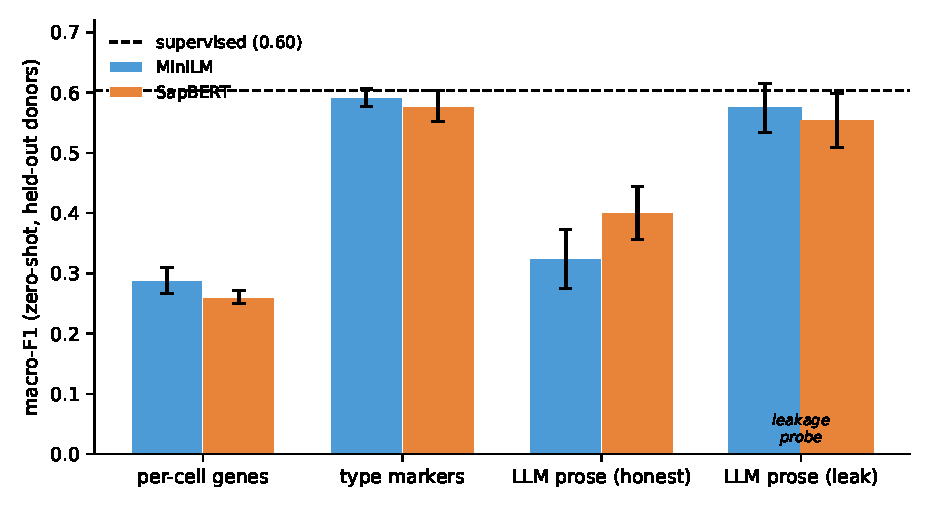
\includegraphics[width=\columnwidth]{figures/fig1_grounding_source.pdf}
  \caption{Zero-shot macro-F1 on held-out donors by grounding source and
  text encoder (mean $\pm$ s.d., 3 seeds). Dashed line: supervised
  cell-only baseline. The hatched group is a leakage probe (type name
  present in LLM prose), not an honest grounding result.}
  \label{fig:main}
\end{figure}

\begin{table}[t]
\centering\small
\begin{tabular}{@{}llllcc@{}}
\toprule
arm & source & encoder & leak & macro-F1 & bal.\ acc \\
\midrule
supervised & --- & --- & & 0.603$\pm$.018 & 0.618$\pm$.017 \\
probe & own genes & MiniLM & & 0.414$\pm$.001 & 0.476$\pm$.025 \\
probe & own genes & SapBERT & & 0.404$\pm$.013 & 0.483$\pm$.031 \\
probe & type markers & MiniLM & & 0.560$\pm$.053 & 0.578$\pm$.047 \\
probe & type markers & SapBERT & & 0.548$\pm$.013 & 0.585$\pm$.018 \\
probe & LLM honest & MiniLM & & 0.531$\pm$.046 & 0.553$\pm$.030 \\
probe & LLM honest & SapBERT & & 0.549$\pm$.029 & 0.572$\pm$.022 \\
probe & LLM labeled & MiniLM & $\dagger$ & 0.510$\pm$.033 & 0.530$\pm$.047 \\
probe & LLM labeled & SapBERT & $\dagger$ & 0.565$\pm$.036 & 0.579$\pm$.029 \\
\midrule
zero-shot & own genes & MiniLM & & 0.288$\pm$.022 & 0.473$\pm$.031 \\
zero-shot & own genes & SapBERT & & 0.261$\pm$.010 & 0.446$\pm$.050 \\
zero-shot & type markers & MiniLM & & \textbf{0.591$\pm$.015} & \textbf{0.635$\pm$.034} \\
zero-shot & type markers & SapBERT & & 0.578$\pm$.025 & 0.620$\pm$.020 \\
zero-shot & LLM honest & MiniLM & & 0.324$\pm$.049 & 0.436$\pm$.059 \\
zero-shot & LLM honest & SapBERT & & 0.401$\pm$.044 & 0.487$\pm$.015 \\
zero-shot & LLM labeled & MiniLM & $\dagger$ & 0.575$\pm$.040 & 0.625$\pm$.023 \\
zero-shot & LLM labeled & SapBERT & $\dagger$ & 0.553$\pm$.045 & 0.601$\pm$.021 \\
\bottomrule
\end{tabular}
\caption{Held-out-donor performance at 85k cells (mean $\pm$ s.d., seeds
0--2). $\dagger$: leakage probes (type name in text); upper bounds, not
honest grounding. Best honest zero-shot in bold.}
\label{tab:main}
\end{table}

\subsection{The grounding source dominates; the text encoder barely matters}

Across every condition, SapBERT $\approx$ MiniLM on gene-list captions ---
a biomedical entity-linking encoder offers no benefit when the caption is a
comma-separated gene list. On natural prose (LLM arms), SapBERT pulls ahead
in zero-shot (+0.08 F1), consistent with domain pretraining helping only
when the text is actually prose. The dominant axis is the grounding
\emph{source}: a $\sim$2$\times$ zero-shot gap between per-cell gene lists
(0.29) and type markers (0.59).

\subsection{Label-free grounding remains the gap}

Honest label-free sources underperform: per-cell gene lists reach 0.29 F1
zero-shot, and LLM prose inferred \emph{from markers alone} --- which
correctly recovered lineage and function (e.g., ``megakaryocyte
developmental continuum'' from \texttt{PPBP, TUBB1, GP9, ITGA2B}) ---
reaches 0.40 with SapBERT. The probe-vs-zero-shot gap
(Figure~\ref{fig:gap}) is instructive: for \texttt{type\_markers} the gap
is \emph{negative} (zero-shot beats the probe), meaning the aligned space
itself carries the discriminative structure; for label-free sources the gap
is positive, i.e., the representation still needs label supervision to be
read out.

\begin{figure}[t]
  \centering
  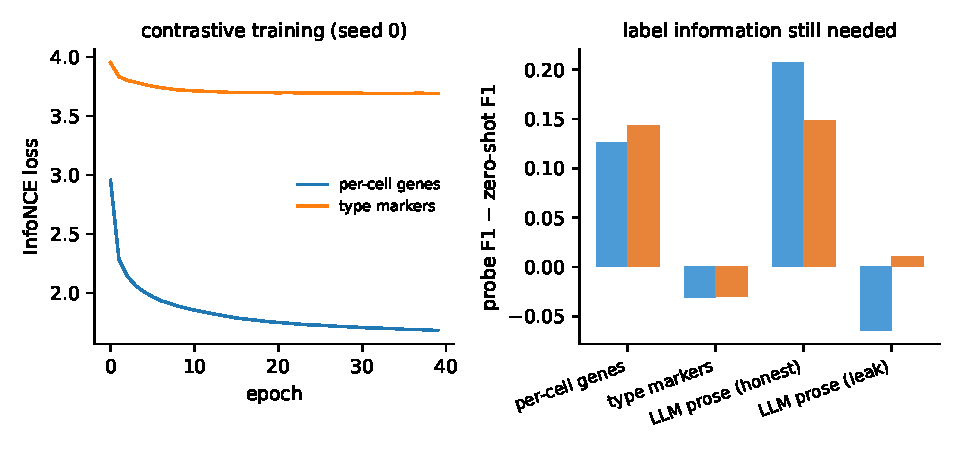
\includegraphics[width=\columnwidth]{figures/fig2_loss_gap.pdf}
  \caption{Left: contrastive training curves (seed 0, MiniLM). The
  \texttt{type\_markers} plateau is expected --- only 16 unique texts, so
  most batch pairs collide. Right: linear-probe minus zero-shot F1 ---
  negative values mean the aligned space classifies better than a labeled
  readout.}
  \label{fig:gap}
\end{figure}

\subsection{Leaky text does not beat clean text}
\label{sec:leak}

The leakage probe (LLM prose containing the type name) scores 0.575
zero-shot --- \emph{below} the clean \texttt{type\_markers} arm. The reason
is format consistency: class captions are marker lists, so train captions
in the same register transfer best. Leakage helps only when train and eval
text share register, underscoring that benchmark comparisons of grounding
methods must control caption \emph{format}, not just label content.

\subsection{External literature retrieval closes most of the label-free gap}
\label{sec:m6}

Table~\ref{tab:m6} reports grounding from text that is external to our
training labels. Under matched-register evaluation, PubMed text retrieved
by marker queries --- with the cell-type name stripped --- reaches 0.563
macro-F1, 95\% of the label-derived \texttt{type\_markers} arm and within
0.04 of the supervised baseline. The end-to-end label-free arm
(curated PanglaoDB markers $\to$ retrieval $\to$ name-stripped text)
reaches 0.512, and curated markers used directly as captions reach 0.459
--- respectively 87\% and 78\% of the label-derived effect, both above
the pre-registered 75\% positive threshold. The register control is
decisive: the \emph{same} retrieved captions evaluated against
marker-list class captions collapse to 0.15--0.19 F1, a $\sim$0.4
penalty attributable purely to caption format. On the retrieval side,
HGNC alias expansion raised pooled candidates by 72\% and
high-marker-coverage documents by 40\%; curated external markers pooled
\emph{more} documents than train-derived markers, so external knowledge
is not recall-limited at this scale.

The strongest honest arm pairs retrieval with LLM synthesis
(\texttt{ragllm\_honest}): Qwen2.5-14B reads the top retrieved excerpts
--- the type name is never shown --- and writes a two-sentence
functional description; outputs that infer a conventional name are
stripped and flagged (2/16, mostly ``megakaryocyte'' inferred from
platelet markers). These descriptions reach 0.589 macro-F1 /
0.631 balanced accuracy --- statistically indistinguishable from both
the label-derived marker arm (0.591/0.635) and the supervised baseline
(0.600/0.620). The labeled synthesis probe (name shown, 0.600) bounds
the residual headroom at $\approx$0.01. Finally, substituting the
PanglaoDB curated markers as the query source (\texttt{ragllm\_curated})
makes the pipeline label-free end-to-end --- external marker database,
external literature, LLM synthesis, name never shown anywhere --- and
reaches \textbf{0.603 macro-F1 / 0.634 balanced accuracy} (SapBERT),
matching the supervised baseline with zero labels in the chain.
Substituting OLMo-2-13B \citep{olmo2} for Qwen2.5-14B in the synthesis
step reproduces the result within noise (honest 0.597, curated
label-free \textbf{0.598}, labeled 0.606 macro-F1), so the finding is
not specific to the synthesis model.

\begin{table}[t]
\centering\small
\begin{tabular}{@{}lllcc@{}}
\toprule
arm & query source & label-free & F1 & bal.\ acc \\
\midrule
\texttt{type\_markers} (M3 ref.) & train labels & no & 0.591 & 0.635 \\
\texttt{extkb\_markers} & PanglaoDB (direct) & yes & 0.459 & 0.564 \\
\texttt{rag\_markers\_alias} & train markers+aliases & text only & 0.563 & 0.613 \\
\texttt{rag\_curated\_alias} & PanglaoDB+aliases & \textbf{yes} & 0.512 & 0.565 \\
\texttt{ragllm\_honest} & retrieval$\to$Qwen synth & text only & 0.589 & 0.631 \\
\texttt{ragllm\_curated} & PanglaoDB$\to$retr.$\to$Qwen & \textbf{yes} & \textbf{0.603} & \textbf{0.634} \\
\texttt{ragllm\_labeled} & name shown to LLM & no (upper bound) & 0.600 & 0.635 \\
\texttt{rag\_name} & type name + MeSH & no (upper bound) & 0.506 & 0.554 \\
\bottomrule
\end{tabular}
\caption{External-knowledge grounding, matched-register zero-shot
(macro-F1 / balanced accuracy, best encoder per arm, held-out donors).
``text only'': retrieved text is external but the query originates from
train-derived markers. All external arms strip the literal type name.}
\label{tab:m6}
\end{table}

\subsection{Identifier semantics: a cautionary engineering finding}
\label{sec:symbols}

Our first benchmark iteration silently produced meaningless captions:
census-downloaded matrices carry feature IDs as \texttt{var\_names}, and
one cached file had \emph{positional} indices (\texttt{"0"}, \texttt{"1"},
\ldots). Captions therefore listed tokens with no biological semantics.
After mapping to gene symbols via \texttt{feature\_name}, honest zero-shot
F1 improved from 0.214 to 0.293 on the 30k benchmark --- a 37\% relative
change from a ``plumbing'' fix. Any language-grounded pipeline that does
not explicitly validate identifier semantics risks the same failure;
we pin it with regression tests.

\subsection{Donor-level pathology representations in SEA-AD}
\label{sec:m8}

We extended the pipeline to the SEA-AD Alzheimer's atlas (240{,}026
nuclei, 127 donors, MTG+V1C) and asked whether embeddings trained to
discriminate cell \emph{identity} carry donor \emph{state}. Mean-pooled
donor embeddings from the M7 cell-type objective exceeded a
pseudobulk-PCA baseline on the continuous cortical pathology score
(CPS; Spearman $\rho \approx 0.4$ vs.\ $0.21$ on held-out donors) but
fell short of our pre-registered gate ($\rho \geq 0.5$) and produced no
consistent ordinal trajectory. Variance analysis explains the ceiling:
$\sim$93\% of embedding variance separates cell types, leaving donor
state as a $\sim$7\% side-channel.

We therefore retrained the contrastive objective against captions
describing each \emph{donor's pathology label} rather than each cell's
type, and swept eight pathology targets (ADNC, Braak, CERAD, Thal,
cognitive status, quantile-binned CPS, and a cell-type$\times$ADNC
composite) under a donor-label-permutation null. On held-out donors,
donor embeddings now reach $\rho = 0.62$ for CPS (binary cognitive
status), $0.52$--$0.57$ for molecular ordinals, with positive Braak /
CERAD / ADNC trajectories for the strongest arms and a $+0.15$--$0.36$
gap over shuffled-label controls. Per-cell pathology classification
remains at chance, confirming that the signal aggregates at the donor
level. Two targets falsified cleanly: Thal phase (label saturation in
this cohort) and the 96-class composite (diluted contrast). The
objective, not the architecture, determines which biology the
representation retains.

Scaling to the full atlas (440{,}390 nuclei across 11 cortical and
hippocampal regions; same 84 donors) preserves the effect: cognitive
status holds $\rho \approx 0.60$ with stable ADNC/CERAD trajectories
($\rho = 0.65$--$0.70$) in both text encoders, and regional transfer
recovers a vulnerability-consistent ordering (MTG $\rho \approx 0.65$ >
STG > MEC > AnG > V1C; hippocampus is an honest outlier at $\sim$0).
The binding constraint is donor count, not cells: 84 unique donors
yields $\sim$21 held-out donors, so further gains require new cohorts
rather than more nuclei per donor.

\subsection{External replication in ROSMAP and cross-cohort transfer}
\label{sec:m11}

We replicated the protocol on the open ROSMAP multiregion snRNA-seq
release \citep{liu2025rosmap}: 300{,}057 nuclei from 111 donors across
six regions (HC, EC, TH, AG, MTC, PFC), downsampled to $\leq$800 cells
per donor$\times$region and embedded in the same 2000-HVG space. The
open release carries a coarse three-level pathology label
(nonAD/earlyAD/lateAD) rather than continuous scores --- we
pre-registered the ordinal level as the replication target and note
this asymmetry throughout.

\paragraph{Replication is partial and target-dependent.}
Donor-held-out training on ROSMAP reproduces the ordinal trajectory
structure (real $\rho = 0.37$ vs.\ shuffled-label null $-0.08$) and,
strikingly, the same region-vulnerability gradient as SEA-AD
(hippocampus $\rho \approx 0.57$ $>$ entorhinal $\approx 0.55$ $>$
cortical regions $\approx 0.3$--$0.4$). However, on this coarse target
the grounded model does \emph{not} beat an expression-only pseudobulk
baseline ($\rho = 0.51$ vs.\ $0.52$) --- unlike SEA-AD, where the same
objective doubled it (0.60 vs.\ 0.26). The grounding advantage is
largest precisely when the phenotype is a fine continuous score that
mean expression dilutes; when the label is a coarse class driven by
compositional shifts, expression alone suffices.

\paragraph{Zero-shot cross-cohort transfer passes the pre-registered
gate.} Sharing the SEA-AD 2000-gene input space, we applied each
cohort's model to the other without fitting anything on the target.
The ROSMAP-trained model --- conditioned only on three-level pathology
captions --- predicts SEA-AD's continuous CPS at $\rho = 0.46$--$0.52$
(bootstrap CIs exclude zero; held-out half of donors), within $\sim$0.1
of the within-cohort models. The reverse direction is weaker
($\rho \approx 0.29$ for ADNC captions, $\approx 0.18$ for binary
cognitive status): transfer toward a continuous target tolerates
partial axis alignment, and cognition and neuropathology are partially
dissociable, consistent with the cognitive-resilience literature. The
transfer result is robust to grounding source: a ROSMAP model grounded
on retrieved PubMed captions instead of authored ones transfers at
$\rho = 0.47$ --- statistically indistinguishable from the manual-caption
transfer --- even though retrieval captions confer no within-cohort gain
on the coarse three-level target ($\rho = 0.43$--$0.44$, still
$\leq$ pseudobulk).

\paragraph{What moves the number: captions, not pooling.}
We swept three improvement avenues on SEA-AD. Gated attention/MIL donor
pooling failed to beat mean pooling (negative result; mean stays). A
soft-ordinal contrastive loss that spreads probability mass over nearby
ordinal captions sharpened ADNC/CERAD trajectories by $+0.04$--$0.10$
at some cost to ridge-CPS signal. The largest gain came from the
grounding corpus itself: replacing manually authored pathology captions
with direct PubMed retrieval (title/abstract concatenation, no LLM
synthesis) lifted CPS to $\rho = 0.60$--$0.61$ on \emph{both} text
encoders ($+0.05$/$+0.13$ over manual captions) --- evidence that
retrieved literature, not engineered prose, is the stronger grounding
source.

\paragraph{Comparison with external foundation models.}
Under the identical donor-held-out protocol without fine-tuning,
pretrained single-cell foundation models trail the pathology-grounded
objective on donor state: scGPT reaches CPS $\rho = 0.43$--$0.51$,
Geneformer V2-104M $0.13$--$0.46$, Geneformer V1-10M $0.28$--$0.37$,
and CellWhisperer $0.34$--$0.58$, versus $0.60$--$0.61$ for the
grounded model. Cell-type identity tells the opposite story ---
foundation models dominate the type probe (up to 0.95 macro-F1) ---
confirming that identity and state are separable axes and that
unsupervised corpus diversity alone does not recover the
pathology-progression axis as efficiently as targeted grounding.

\section{Discussion under revalidation}

\paragraph{Supervision is not semantic attribution.}
Class annotations determine the training cell--caption pairs, including the
external-marker and name-stripped arms. Their results therefore concern
text-mediated supervision, not label-free training. Fixed random and one-hot
class prototypes and non-text objectives with the same labels are required to
identify any additional contribution of biological semantics. Matched-register
performance also needs testing against independently phrased class descriptions.

\paragraph{Composition and state remain unresolved.}
A donor mean mixes cell-type and regional proportions with within-group states.
The historical composition correlation near 0.50 is an important baseline, but
subtracting it from an embedding correlation near 0.61 does not isolate state
information. Train-only scaling, covariate adjustment, within-type/region
analysis and paired donor-level comparisons are specified in ADR-011. Sampled
nucleus fractions do not establish absolute cell loss or causal vulnerability.

\paragraph{Transfer and encoder scale.}
The historical transfer procedure fits PCA in the target cohort and uses an
orientation subset's labels. It should be distinguished from a source-fitted
predictor evaluated without target fitting or labels. Likewise, the negative
scGPT sweep concerns the configurations and training budgets tested, not a
general absence of benefit from encoder capacity. Native tokenization and
matched cells, probes and budgets are prerequisites for foundation-model claims.

\paragraph{Biological and statistical limitations.}
The study spans blood and post-mortem brain cohorts and uses both Qwen and OLMo
for synthesis. Nevertheless, independent sample sizes are donor counts, not
cell counts; repeated model selection on the same splits remains exploratory.
The open ROSMAP matrix exposes a coarse three-level endpoint unlike continuous
SEA-AD CPS. CPS denotes a Continuous Pseudoprogression Score derived from
quantitative neuropathology, not longitudinal observation of disease progression.
Caption discrimination is not proof of biological correctness: the audit found
incorrect lineage assertions in generated descriptions. Domain review, source
support, paired confidence intervals, matched permutation controls and explicit
handling of incomplete gates remain necessary before submission.

\section{Conclusion}

Historical experiments motivate a controlled study of text-mediated
supervision across cell identity and donor pathology. They do not yet establish
an advantage attributable specifically to biological language, a causal
composition/state decomposition, or strict zero-shot cohort transfer. The next
step is methodological revalidation with equivalent supervision, frozen data
contracts, inductive transforms and donor-level uncertainty, rather than
additional model complexity. Final claims and the submission-ready manuscript
will be determined by those comparisons, including negative outcomes.

\bibliographystyle{plainnat}
\bibliography{refs}

\end{document}
